% Options for packages loaded elsewhere
\PassOptionsToPackage{unicode}{hyperref}
\PassOptionsToPackage{hyphens}{url}
%
\documentclass[
  oneside]{article}
\usepackage{amsmath,amssymb}
\usepackage{iftex}
\ifPDFTeX
  \usepackage[T1]{fontenc}
  \usepackage[utf8]{inputenc}
  \usepackage{textcomp} % provide euro and other symbols
\else % if luatex or xetex
  \usepackage{unicode-math} % this also loads fontspec
  \defaultfontfeatures{Scale=MatchLowercase}
  \defaultfontfeatures[\rmfamily]{Ligatures=TeX,Scale=1}
\fi
\usepackage{lmodern}
\ifPDFTeX\else
  % xetex/luatex font selection
\fi
% Use upquote if available, for straight quotes in verbatim environments
\IfFileExists{upquote.sty}{\usepackage{upquote}}{}
\IfFileExists{microtype.sty}{% use microtype if available
  \usepackage[]{microtype}
  \UseMicrotypeSet[protrusion]{basicmath} % disable protrusion for tt fonts
}{}
\makeatletter
\@ifundefined{KOMAClassName}{% if non-KOMA class
  \IfFileExists{parskip.sty}{%
    \usepackage{parskip}
  }{% else
    \setlength{\parindent}{0pt}
    \setlength{\parskip}{6pt plus 2pt minus 1pt}}
}{% if KOMA class
  \KOMAoptions{parskip=half}}
\makeatother
\usepackage{xcolor}
\usepackage{color}
\usepackage{fancyvrb}
\newcommand{\VerbBar}{|}
\newcommand{\VERB}{\Verb[commandchars=\\\{\}]}
\DefineVerbatimEnvironment{Highlighting}{Verbatim}{commandchars=\\\{\}}
% Add ',fontsize=\small' for more characters per line
\usepackage{framed}
\definecolor{shadecolor}{RGB}{248,248,248}
\newenvironment{Shaded}{\begin{snugshade}}{\end{snugshade}}
\newcommand{\AlertTok}[1]{\textcolor[rgb]{0.94,0.16,0.16}{#1}}
\newcommand{\AnnotationTok}[1]{\textcolor[rgb]{0.56,0.35,0.01}{\textbf{\textit{#1}}}}
\newcommand{\AttributeTok}[1]{\textcolor[rgb]{0.13,0.29,0.53}{#1}}
\newcommand{\BaseNTok}[1]{\textcolor[rgb]{0.00,0.00,0.81}{#1}}
\newcommand{\BuiltInTok}[1]{#1}
\newcommand{\CharTok}[1]{\textcolor[rgb]{0.31,0.60,0.02}{#1}}
\newcommand{\CommentTok}[1]{\textcolor[rgb]{0.56,0.35,0.01}{\textit{#1}}}
\newcommand{\CommentVarTok}[1]{\textcolor[rgb]{0.56,0.35,0.01}{\textbf{\textit{#1}}}}
\newcommand{\ConstantTok}[1]{\textcolor[rgb]{0.56,0.35,0.01}{#1}}
\newcommand{\ControlFlowTok}[1]{\textcolor[rgb]{0.13,0.29,0.53}{\textbf{#1}}}
\newcommand{\DataTypeTok}[1]{\textcolor[rgb]{0.13,0.29,0.53}{#1}}
\newcommand{\DecValTok}[1]{\textcolor[rgb]{0.00,0.00,0.81}{#1}}
\newcommand{\DocumentationTok}[1]{\textcolor[rgb]{0.56,0.35,0.01}{\textbf{\textit{#1}}}}
\newcommand{\ErrorTok}[1]{\textcolor[rgb]{0.64,0.00,0.00}{\textbf{#1}}}
\newcommand{\ExtensionTok}[1]{#1}
\newcommand{\FloatTok}[1]{\textcolor[rgb]{0.00,0.00,0.81}{#1}}
\newcommand{\FunctionTok}[1]{\textcolor[rgb]{0.13,0.29,0.53}{\textbf{#1}}}
\newcommand{\ImportTok}[1]{#1}
\newcommand{\InformationTok}[1]{\textcolor[rgb]{0.56,0.35,0.01}{\textbf{\textit{#1}}}}
\newcommand{\KeywordTok}[1]{\textcolor[rgb]{0.13,0.29,0.53}{\textbf{#1}}}
\newcommand{\NormalTok}[1]{#1}
\newcommand{\OperatorTok}[1]{\textcolor[rgb]{0.81,0.36,0.00}{\textbf{#1}}}
\newcommand{\OtherTok}[1]{\textcolor[rgb]{0.56,0.35,0.01}{#1}}
\newcommand{\PreprocessorTok}[1]{\textcolor[rgb]{0.56,0.35,0.01}{\textit{#1}}}
\newcommand{\RegionMarkerTok}[1]{#1}
\newcommand{\SpecialCharTok}[1]{\textcolor[rgb]{0.81,0.36,0.00}{\textbf{#1}}}
\newcommand{\SpecialStringTok}[1]{\textcolor[rgb]{0.31,0.60,0.02}{#1}}
\newcommand{\StringTok}[1]{\textcolor[rgb]{0.31,0.60,0.02}{#1}}
\newcommand{\VariableTok}[1]{\textcolor[rgb]{0.00,0.00,0.00}{#1}}
\newcommand{\VerbatimStringTok}[1]{\textcolor[rgb]{0.31,0.60,0.02}{#1}}
\newcommand{\WarningTok}[1]{\textcolor[rgb]{0.56,0.35,0.01}{\textbf{\textit{#1}}}}
\usepackage{graphicx}
\makeatletter
\def\maxwidth{\ifdim\Gin@nat@width>\linewidth\linewidth\else\Gin@nat@width\fi}
\def\maxheight{\ifdim\Gin@nat@height>\textheight\textheight\else\Gin@nat@height\fi}
\makeatother
% Scale images if necessary, so that they will not overflow the page
% margins by default, and it is still possible to overwrite the defaults
% using explicit options in \includegraphics[width, height, ...]{}
\setkeys{Gin}{width=\maxwidth,height=\maxheight,keepaspectratio}
% Set default figure placement to htbp
\makeatletter
\def\fps@figure{htbp}
\makeatother
\setlength{\emergencystretch}{3em} % prevent overfull lines
\providecommand{\tightlist}{%
  \setlength{\itemsep}{0pt}\setlength{\parskip}{0pt}}
\setcounter{secnumdepth}{-\maxdimen} % remove section numbering
\newlength{\cslhangindent}
\setlength{\cslhangindent}{1.5em}
\newlength{\csllabelwidth}
\setlength{\csllabelwidth}{3em}
\newlength{\cslentryspacingunit} % times entry-spacing
\setlength{\cslentryspacingunit}{\parskip}
\newenvironment{CSLReferences}[2] % #1 hanging-ident, #2 entry spacing
 {% don't indent paragraphs
  \setlength{\parindent}{0pt}
  % turn on hanging indent if param 1 is 1
  \ifodd #1
  \let\oldpar\par
  \def\par{\hangindent=\cslhangindent\oldpar}
  \fi
  % set entry spacing
  \setlength{\parskip}{#2\cslentryspacingunit}
 }%
 {}
\usepackage{calc}
\newcommand{\CSLBlock}[1]{#1\hfill\break}
\newcommand{\CSLLeftMargin}[1]{\parbox[t]{\csllabelwidth}{#1}}
\newcommand{\CSLRightInline}[1]{\parbox[t]{\linewidth - \csllabelwidth}{#1}\break}
\newcommand{\CSLIndent}[1]{\hspace{\cslhangindent}#1}
\ifLuaTeX
\usepackage[bidi=basic]{babel}
\else
\usepackage[bidi=default]{babel}
\fi
\babelprovide[main,import]{spanish}
% get rid of language-specific shorthands (see #6817):
\let\LanguageShortHands\languageshorthands
\def\languageshorthands#1{}
\usepackage{makeidx}
\makeindex
\usepackage{graphicx}
\usepackage{tikz}
\usepackage{atbegshi}


\AtBeginDocument{
    \AtBeginShipoutNext{
        \AtBeginShipoutUpperLeft{
            \put(\dimexpr\paperwidth/2-\textwidth/2\relax, -650){
                \makebox[\textwidth]{
                    
\includegraphics[width=0.45\textwidth]{cure_udelar.png}  % Adjust width as needed
                    \hfill
                    
\includegraphics[width=0.405\textwidth]{logoMEDIA.jpeg} % Make it 90% smaller
                }
            }
        }
    }
}
\ifLuaTeX
  \usepackage{selnolig}  % disable illegal ligatures
\fi
\IfFileExists{bookmark.sty}{\usepackage{bookmark}}{\usepackage{hyperref}}
\IfFileExists{xurl.sty}{\usepackage{xurl}}{} % add URL line breaks if available
\urlstyle{same}
\hypersetup{
  pdftitle={Entrega: curso de datos extremales},
  pdfauthor={Laura Montaldo, CI: 3.512.962-7},
  pdflang={es},
  hidelinks,
  pdfcreator={LaTeX via pandoc}}

\title{Entrega: curso de datos extremales}
\author{Laura Montaldo, CI: 3.512.962-7}
\date{2024-02-29}

\begin{document}
\maketitle

\newpage

\thispagestyle{empty}

\maketitle

\newpage

\tableofcontents

\newpage

\hypertarget{resumen}{%
\section{Resumen}\label{resumen}}

Your abstract goes here.

\newpage

\chapter{Motivación y objetivo del estudio}

Los índices de \(S\&P\) son una familia de índices de renta
variable\footnote{En inglés se llaman equity indices} diseñados para
medir el rendimiento del mercado de acciones en Estados Unidos que
cotizan en bolsas estadounidenses. Ésta familia de índices está
compuesta por una amplia variedad de índices basados en tamaño, sector y
estilo. Los índices están ponderados por el criterio
\textit{float-adjusted market capitalization} (FMC). Además, se disponen
de índices ponderados de manera equitativa y con límite de
capitalización de mercado, como es el caso del \(S\&P\:500\). Este este
sentido, el \(S\&P 500\) entraría en el conjunto de índices ponderados
por capitalización bursátil ajustada a la flotación (ver
\href{http://www.overleaf.com}{\textcolor{blue}{$S\&P$ Dow Jones Indices}}).
El mismo mide el rendimiento del segmento de gran capitalización del
mercado estadounidense. Es considerado como un indicador representativo
del mercado de renta variable de los Estados Unidos, y está compuesto
por 500 empresas constituyentes.

Se busca crear un indicador de una posible crisis bursátil. Como
variable de referencia de toma la relación de precios al cierre de ayer
sobre la de hoy

\begin{equation}
Indicador_t=\frac{Precio_{t-1}}{Precio_t},\quad\text{para}\; t=1,...,T \label{eq:ind}
\end{equation} \vspace{0.5cm}

Interpretación del Indicador:

\begin{itemize}
\item Si el $Indicador_t$    $\leq$ 1, el precio de cierre de hoy es mayor o igual que el de ayer, lo cual podría ser considerado una señal positiva.
\item Si el $Indicador_t$ > 1, el precio de cierre de hoy es menor que el de ayer, lo cual podría considerarse una señal de alerta.
\end{itemize}

\vspace{1cm}

En las siguiente figura @ref(fig:plot1) se muestra la evolución
histórica desde la fecha 03/01/1928 hasta 08/12/2023 del precio al
cierre del día del indicar S\&P 500.

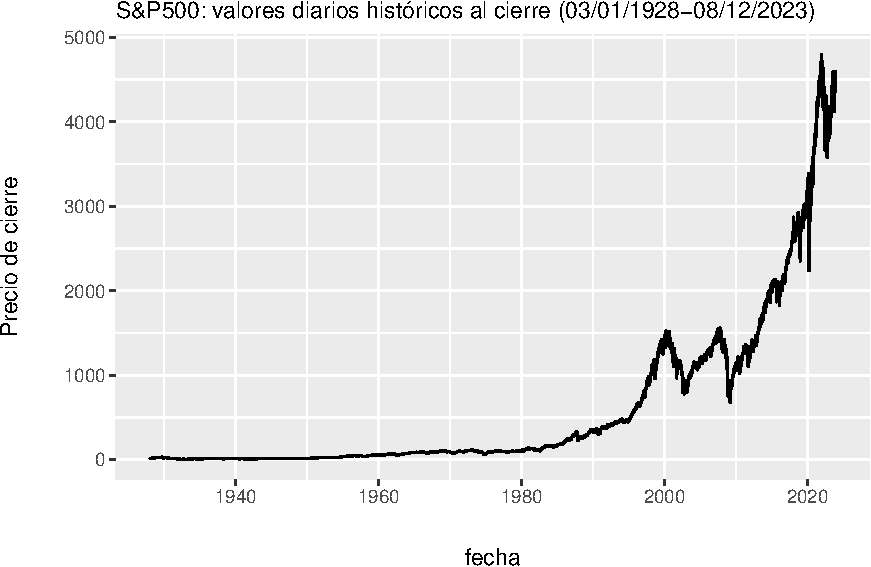
\includegraphics{Entrega_Laura_Montaldo_files/figure-latex/plot1-1.pdf}

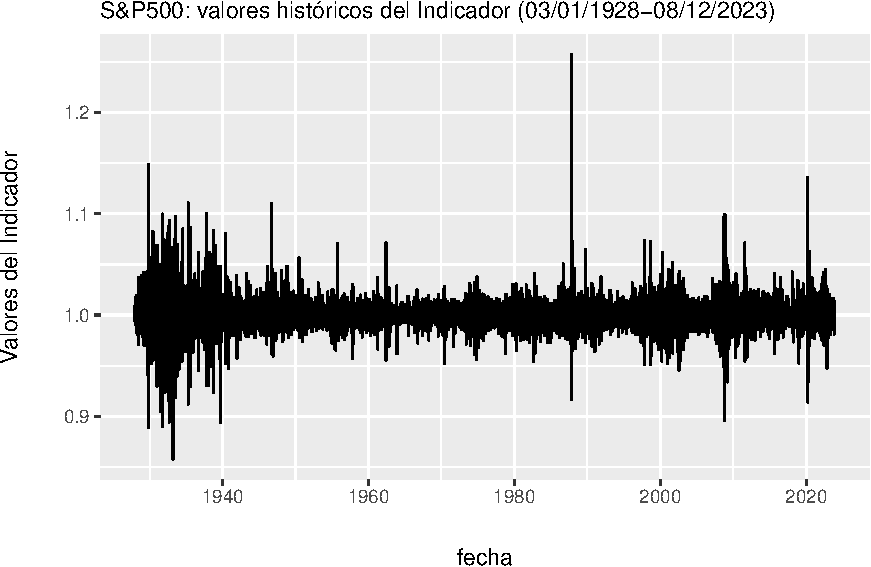
\includegraphics{Entrega_Laura_Montaldo_files/figure-latex/plot2-1.pdf}
\newpage

\chapter{Marco Teórico}

\section{Capítulo 1: Teoría asintótica clásica y las distribuciones extremales y sus dominios de atracción}
\subsection{Distrubiciones extremales}

Cuando tomamos los máximos de las variables \(iid\) con un rango
acotado, la distribución resultante por la cual se puede aproximar es la
de Weibull.

\begin{Shaded}
\begin{Highlighting}[]
\FunctionTok{head}\NormalTok{(df)}
\end{Highlighting}
\end{Shaded}

\begin{verbatim}
##         Date  Open  High   Low Close Volume Dividends Stock.Splits  relacion
## 2 1928-01-03 17.76 17.76 17.76 17.76      0         0            0 0.9943693
## 3 1928-01-04 17.72 17.72 17.72 17.72      0         0            0 1.0022574
## 4 1928-01-05 17.55 17.55 17.55 17.55      0         0            0 1.0096866
## 5 1928-01-06 17.66 17.66 17.66 17.66      0         0            0 0.9937712
## 6 1928-01-09 17.50 17.50 17.50 17.50      0         0            0 1.0091428
## 7 1928-01-10 17.37 17.37 17.37 17.37      0         0            0 1.0074841
\end{verbatim}

\hypertarget{refs}{}
\begin{CSLReferences}{1}{0}
\leavevmode\vadjust pre{\hypertarget{ref-notas_curso}{}}%
Perera, Gonzalo, Angel Segura, y Carolina Crisci. 2021. \emph{Curso de
estadística de datos extremales, cap. 1 a cap. 5}.

\leavevmode\vadjust pre{\hypertarget{ref-evd}{}}%
Stephenson, A. G. 2002. {«evd: Extreme Value Distributions»}. \emph{R
News} 2 (2): 0. \url{https://CRAN.R-project.org/doc/Rnews/}.

\end{CSLReferences}

\end{document}
